%\documentclass[11pt,a4paper]{article}
\documentclass[11pt,a4paper]{scrartcl}
%\documentclass[11pt,a4paper,oneside]{book}
\usepackage[british,UKenglish,USenglish,english,american]{babel}
%\usepackage[a4paper, total={16cm, 23cm}]{geometry}
\usepackage[tmargin = 1in,bmargin = 1in,lmargin = 0.75in,rmargin = 
0.75in]{geometry}
\usepackage{tikz}
\usepackage{graphicx}
\usepackage{pgfplots}
\pgfplotsset{width=12cm,compat=1.9}
\usepackage{setspace}
\usepackage{chemmacros}
\usepackage{chemfig}
%\usepackage{ghsystem}
\usechemmodule{reactions}
%\usepackage{chemnum}
%\usepackage{bohr}
%\usepackage{elements}
%\usepackage{endiagram}
%\usepackage{modiagram}
%\usepackage{chemgreek}
%\usepackage{mhchem}
\usepackage{esint}
\usepackage{tabularray}

\usepackage{makeidx}
\usepackage{epstopdf}

\usepackage{amssymb}
\usepackage{mathrsfs}
%\usepackage{minted}
\usepackage{bm}
\usepackage{amsmath}
\usepackage{enumitem}
\usepackage[english]{varioref}
\usepackage[english]{babel}
\usepackage{lipsum}
\usepackage{fancyhdr}
\pagestyle{fancy} 
\usepackage{float}
\usepackage{empheq}
\usepackage[framemethod=tikz]{mdframed}
\usepackage{epstopdf}
\numberwithin{equation}{section}
\usepackage{eso-pic}
\usepackage{calc}
\usepackage{nccmath}
\usepackage{caption}
\usepackage{subcaption}
\usepackage{gensymb}
\usepackage{amsfonts,amsthm,epsfig,epstopdf,titling,url,array}
\usepackage{siunitx}
\sisetup{input-digits = 0123456789\pi}
\usepackage[symbol]{footmisc}
\usepackage{xcolor}
\usepackage{multicol}
\usepackage{boondox-cal}
\DeclareSIUnit\atm{atm}
\setcounter{secnumdepth}{3}
\setcounter{tocdepth}{3}
\usepackage{booktabs}
\usepackage{blindtext}
\usepackage{changepage}
\usepackage{longtable}

% \usepackage{draftwatermark}
% \SetWatermarkText{DRAFT}
% \SetWatermarkScale{5}

\DeclareSIUnit\atm{atm}


\pagestyle{fancy} 
\fancypagestyle{firstpage}{
\rhead{
%	\begin{picture}(0,0) 
%			\put(-30,0){\includegraphics[width=1cm]{figures/MCI_4C_bw.eps}} 
%	\end{picture}
}
}
\fancyhead[L]{\slshape\nouppercase{\leftmark}}
\chead{}
\rhead{
%	\begin{picture}(0,0) 
%		\put(-30,0){\includegraphics[width=1cm]{figures/MCI_4C_bw.eps}} 
%	\end{picture}
}
\lfoot{\textit{}}
\cfoot{-\ \thepage\ -}
\rfoot{\textit{}}

\DeclareMathOperator{\rank}{rank}
\DeclareMathOperator{\atantwo}{atan2}
\DeclareMathOperator{\spn}{span}

\renewcommand{\headrulewidth}{0.4pt}
\renewcommand{\footrulewidth}{0.4pt}
\newcommand{\abs}[1]{\left|#1\right|}
\definecolor{mycolor1}{rgb}{0.97, 0.97, 0.97}
\definecolor{mycolor2}{rgb}{0.97, 0.97, 0.97}
\definecolor{tableShade}{gray}{0.9}
\newcommand{\sign}{\text{sign}}
\newcommand{\centered}[1]{\begin{tabular}{@{}l@{}} #1 \end{tabular}}
\theoremstyle{it}

%\newtheorem{defn}{Definition}[chapter]
%\newtheorem{assumption}{Assumption}[chapter]
%\newtheorem{thm}{Theorem}[chapter]
%\newtheorem{lemma}{Lemma}[chapter]
%\newtheorem{corollary}{Corollary}[chapter]

\newtheorem{defn}{Definition}[section]
\newtheorem{assumption}{Assumption}[section]
\newtheorem{thm}{Theorem}[section]
\newtheorem{lemma}{Lemma}[section]
\newtheorem{corollary}{Corollary}[section]


\theoremstyle{definition}
%\theoremstyle{it}
\newtheorem{example}{Example}[section]

\newenvironment{myitemize_1}
{ \begin{itemize}[topsep=0pt]
		\setlength{\topsep}{2pt}		
		\setlength{\itemsep}{2pt}
		\setlength{\parskip}{2pt}
		\setlength{\parsep}{2pt}     }
	{ \end{itemize}                  }

\newmdenv[innerlinewidth=0.5pt, roundcorner=4pt,backgroundcolor=mycolor2, 
linecolor=mycolor1,innerleftmargin=6pt,
innerrightmargin=6pt,innertopmargin=6pt,innerbottommargin=6pt]{mybox}

\title{\textbf{ 
	\begin{LARGE}
		Solid State Transformers:
	\end{LARGE} \\[12pt]
	\begin{large}
	architecture, control and simulation results.
	\end{large}
	}
}
\author{\textbf{Davide Bagnara}}

\begin{document}
	\thispagestyle{firstpage}
	\begin{mybox}
		\maketitle
		\vspace{100mm}
	\end{mybox}
	\newpage
	\tableofcontents
	\listoffigures	
	\listoftables
	\newpage

\begin{onehalfspace}
\begin{abstract}
	\begin{adjustwidth}{50pt}{50pt}
		\textit{This document presents a preliminary analysis of Solid State Transformers (SSTs), aiming to provide a comprehensive introduction to the technology. The study proposes some potential layouts for hardware architectures and control strategies, supported by Simscape modeling and simulation results. Furthermore, the document evaluates the capabilities of the Simscape models implemented for this investigation.}
	\end{adjustwidth}
\end{abstract}	

\section{Introduction}
\textbf{Solid State Transformers (SSTs)} are advanced power electronic devices designed to replace traditional low-frequency transformers in modern power distribution systems. By operating at high frequency and using fully controllable conversion stages, SSTs achieve a more compact size, improved energy efficiency, and enhanced functionality compared to conventional transformers. Beyond simple voltage transformation, they provide additional services such as bidirectional power flow, voltage and reactive power regulation, and seamless integration of distributed energy resources including renewables, electric vehicles, and energy storage.

A key difference from traditional transformers is the behavior of SSTs during fault conditions. Due to their electronic nature and active current limiting, SSTs inherently restrict short-circuit currents. This prevents downstream systems from relying on conventional overcurrent-based protection schemes, which depend on high fault currents for detection. As a result, new protection strategies based on advanced sensing, high-speed control, and intelligent fault identification must be implemented. This shift in protection philosophy presents both challenges and significant opportunities for the development of more flexible, reliable, and smart power networks.

\section{Global Architecture}
In this chapter few general architectures for SST solutions are proposed and investigated; the SST device is intended to operate between two different grids:
\begin{itemize}
	\item[--] a low voltage DC grid source where many contributors can be assumed are connected e.g. energy storage, photovoltaic installations, car chargers and others;
	\item[--] a three phase medium voltage AC grid source;	 
\end{itemize} 

\noindent Figure~\ref{sst_design_ctrl_fig4b} shows a single phase architecture, which basically consists by a cascade of single phase inverters, where each single phase inverter is supplied by a galvanically isolated DC/DC converter. Each single phase inverter which constitute a single are all connected in series to achieve the selected AC medium voltage; on the other hand all DC/DC input stage are connected in parallel.

\noindent\textbf{Remark} - to reduce the stress in term of voltage isolation, the HV/MV transformer could be built in a way to equally distribute the phase to grand voltage, as shown in Figure~\ref{sst_design_ctrl_fig4b}.

\noindent\textbf{Remark} - from control point of view the following layout can be assumed:
\begin{itemize}
	\item[--] DC/DC power supply control is monolithic and atomic; 	
	\item[--] three phase active front end (AFE) control architecture can be assumed as follows
	\begin{itemize}
		\item[--] master/slave configuration: for each phase one single phase inverter will be identified as \textit{master} while \textit{slave} the others;		
		\item[--] each single phase inverter is equipped by a single phase PLL (both \textit{master} and \textit{slaves});
		\item[--] an inverter current control (running on \textit{master});		
		\item[--] a voltage controlled source mode (on \textit{slaves}).			
	\end{itemize}
\end{itemize}
\begin{figure}[H]
	\centering
	\includegraphics[width = 500pt, angle = 0, 
	keepaspectratio]{figures/arch/sst_design_ctrl_fig4b.eps}
	\captionsetup{width=0.5\textwidth, font=small}
	\caption{Single phase architecture based on galvanically isolated single phase inverter cascade.}
	\label{sst_design_ctrl_fig4b}
\end{figure}
Figure~\ref{sst_design_ctrl_fig4c} shows a case scenario of global three phase architecture with a common communication bus which performs a global distributed control.

\noindent\textbf{Remark} - a deterministic, Ethernet based, bus controller plays a fundamental role in the \textit{concerto} of the overall system.

\begin{figure}[H]
	\centering
	\includegraphics[width = 500pt, angle = 0, 
	keepaspectratio]{figures/arch/sst_design_ctrl_fig4c.eps}
	\captionsetup{width=0.5\textwidth, font=small}
	\caption{Global architecture for three phase system where a cascade of master/slaves single phase inverter implements the the single phase MV.}
	\label{sst_design_ctrl_fig4c}
\end{figure}

As already mentioned, the aim of this work is to evaluate the performance of different architecture and compare them. For this purpose, single phase inverter will be investigate both by a three levels NPC and three levels T-type as shown in Figure~\ref{sst_design_ctrl_fig1b} and Figure~\ref{single_phase_inverter_ttype}. NPC solution permits to use lower voltage rated IGBT components while T-type will result in a more efficient conversion. 

\noindent\textbf{Remark} - DC-voltage rate is assumed at $U_{dc}^{\text{nom}}\SI{800}{\volt}$.

\begin{figure}[H]
	\centering
	\includegraphics[width = 450pt, angle = 0, 
	keepaspectratio]{figures/arch/sst_design_ctrl_fig1b.eps}
	\captionsetup{width=0.5\textwidth, font=small}
	\caption{Single phase inverter stage: based on three level NPC.}
	\label{sst_design_ctrl_fig1b}
\end{figure}

\begin{figure}[H]
	\centering
	\includegraphics[width = 450pt, angle = 0, 
	keepaspectratio]{figures/arch/single_phase_inverter_ttype.eps}
	\captionsetup{width=0.5\textwidth, font=small}
	\caption{Single phase inverter stage: based on three level T-type.}
	\label{single_phase_inverter_ttype}
\end{figure}

\noindent\textbf{Remark} - concerning the galvanically isolated DC/DC converters the following architecture will be investigated:
\begin{itemize}
	\item[--] three phase DAB;
	\item[--] single phase bidirectional CLLC;
	\item[--] single phase DAB;
\end{itemize} 

\noindent\textbf{Remark} - three phase DAB could have a better behaviour in terms of DC-current controllability, even if the topic will be more further investigated.

\begin{figure}[H]
	\centering
	\includegraphics[width = 540pt, angle = 0, 
	keepaspectratio]{figures/arch/sst_design_ctrl_fig2.eps}
	\captionsetup{width=0.5\textwidth, font=small}
	\caption{Single phase DAB.}
	\label{sst_design_ctrl_fig2}
\end{figure}
\begin{figure}[H]
	\centering
	\includegraphics[width = 540pt, angle = 0, 
	keepaspectratio]{figures/arch/sst_design_ctrl_fig2c.eps}
	\captionsetup{width=0.5\textwidth, font=small}
	\caption{Single phase bidirectional CLLC.}
	\label{sst_design_ctrl_fig2c}
\end{figure}
\begin{figure}[H]
	\centering
	\includegraphics[width = 540pt, angle = 0, 
	keepaspectratio]{figures/arch/sst_design_ctrl_fig2b.eps}
	\captionsetup{width=0.5\textwidth, font=small}
	\caption{Three phase DAB.}
	\label{sst_design_ctrl_fig2b}
\end{figure}






\section{Control Architecture}
The main goal for an SST architecture should be, on one side, to keep stable a DC-grid composted by many \textit{producers/consumers}, and to give an additional stability contribution to the AC-grid vy proper absorbing/generating both reactive as well as active power (assuming DC-grid is integrated by energy storage systems).

Diving into the inner SST control architecture, it is assumed that each DC/DC converter provides a controlled (stable at a given value) DClink voltage, $u_2^{dc}(t) = u_2^{dc}\Big|_{ref}$, while the single phase inverter will drive a current to the AC-grid according to an outer control level\footnote{The outer control loop here intended concerns a global strategy which unified the stability of the DC-grid as well as the stability of the AC-grid according to, e.g. an optimal control based strategy.}, as shown in Figure~\ref{sst_design_ctrl_fig3} shows a possible control principle.
\begin{figure}[H]
	\centering
	\includegraphics[width = 425pt, angle = 0, 
	keepaspectratio]{figures/arch/sst_design_ctrl_fig3.eps}
	\captionsetup{width=0.5\textwidth, font=small}
	\caption{Fundamental control strategies of the isolated single phase inverter.}
	\label{sst_design_ctrl_fig3}
\end{figure}

\subsection{DC/DC Control Loops}
DC/DC control is basically constructed by a cascade of PI-control with an outer voltage loop control followed by an inner current control loop;

\noindent\textbf{Remark} - ZVS condition, for the single phase DAB, is achieved with a dead-time of $t_{dt} = \SI{400}{\nano\second}$.

\noindent\textbf{Remark} - ZVC condition, for the CLLC, is achieved forcing DCM.

\subsection{Single Phase Lock Loop}
Single phase inverter uses a single phase lock loop as shown in Figure~\ref{single_phase_pll_fig1}

\begin{figure}[H]
	\centering
	\includegraphics[width = 425pt, angle = 0, 
	keepaspectratio]{figures/control/single_phase_pll_fig1.eps}
	\captionsetup{width=0.5\textwidth, font=small}
	\caption{Single phase lock loop for grid phase estimation.}
	\label{single_phase_pll_fig1}
\end{figure}


\subsection{Single Phase Inverter Control Layouts}
Single phase inverter has been simulated with resonant PI as well as with virtual vector control as shown in Figure~\ref{single_phase_afe_control_1}

\begin{figure}[H]
	\centering
	\includegraphics[width = 500pt, angle = 0, 
	keepaspectratio]{figures/control/single_phase_afe_control_1.eps}
	\captionsetup{width=0.5\textwidth, font=small}
	\caption{Control layout of the single phase inverter. Same strategy for T-Type.}
	\label{single_phase_afe_control_1}
\end{figure}

\section{Simulation results}
In this section simulation results of the architecture based on three phase DAB is shown, in particular the following operative conditions have been accounted:
\begin{itemize}
	\item[--] three phase DAB works at fundamental frequency of $f_{dab} = \SI{4}{\kilo\hertz}$;	
	\item[--] single phase CLLC works at fundamental frequency of $f_{llc} = \SI{13}{\kilo\hertz}$;
	\item[--] single phase DAB works at fundamental frequency of $f_{spdab} = \SI{12}{\kilo\hertz}$;
	\item[--] single phase inverter operates at the switching frequency of  $f_{inv}^{pwm} = \SI{4}{\kilo\hertz}$, both NPC and T-Type.
\end{itemize}

\noindent\textbf{Remark} - the following switching devices have been used selected
\begin{itemize}
	\item[--] Wolfspeed \textbf{CAB450M12XM3} for the three phase DAB;
	\item[--] Wolfspeed \textbf{CAB760M12HM3} for the single phase DAB and CLLC;
	\item[--] Wolfspeed \textbf{CAB760M12HM3} for the NPC (the number of paralleled device is two);
	\item[--] Wolfspeed \textbf{CAB760M12HM3} + \textbf{CLB800M12HM3P} for the T-Tpype (the number of paralleled device is two);
\end{itemize}

According to Figure~\ref{sst_design_ctrl_fig2c} and Figure~\ref{sst_design_ctrl_fig1b}, the following components shall be accounted:
\begin{itemize}
	\item[--] $L_{Fi}^{dc} = \SI{400}{\micro\henry}$ - input DAB inductance with nominal current of $I_{LFu}^{nom} = \SI{325}{\ampere}$;
	\item[--] $C_{1}^{dc} = \SI{3.6}{\milli\farad}$ - input DAB capacitor with nominal voltage of $U_{dc1}^{nom} = \SI{800}{\volt}$;
	\item[--] $C_{2}^{dc} = \SI{3.6}{\milli\farad}$ - output DAB capacitor with nominal voltage of $U_{dc2}^{nom} = \SI{800}{\volt}$;
	\item[--] $C_{dc}^{inv} = \SI{3.6}{\milli\farad}$ - single phase DClink capacitor, with nominal voltage of $U_{dc}^{nom} = \SI{400}{\volt}$;
	\item[--] $L_{Fu}^{ac} = \SI{300}{\micro\henry}$ - output single phase inverter inductance with nominal current $I_{LFu}^{nom} = \SI{1000}{\ampere}$;
	\item[--] $C_{Fu}^{ac} = \SI{360}{\micro\henry}$ - output single phase inverter capacitor with nominal voltage of $U_{CFu}^{nom} = \SI{270}{\volt}$;
	\item[--] $L_s = \SI{28}{\micro\henry}$ - three phase DAB inductance (this value takes into account also the leakage inductance of the transformer) with nominal current of $I_{Ls}^{nom} = \SI{250}{\ampere}$ at nominal frequency of $f_{Ls}^{nom} = \SI{4}{\kilo\hertz}$;
	\item[--] $L_s = \SI{11}{\micro\henry}$ - single phase DAB inductance (this value takes into account also the leakage inductance of the transformer) with nominal current of $I_{Ls}^{nom} = \SI{400}{\ampere}$ at nominal frequency of $f_{Ls}^{nom} = \SI{12}{\kilo\hertz}$;
	\item[--] $L_s = \SI{13}{\micro\henry}$ - single phase CLLC inductance (this value takes into account also the leakage inductance of the transformer) with nominal current of $I_{Ls}^{nom} = \SI{450}{\ampere}$ at nominal frequency of $f_{Ls}^{nom} = \SI{13}{\kilo\hertz}$;
	\item[--] $C_{s1} = C_{s2} = \SI{10}{\micro\farad}$ - single phase CLLC resonant capacitor ($f_{res} = \SI{20}{\kilo\hertz}$) with nominal current of $I_{Cs}^{nom} = \SI{450}{\ampere}$;
\end{itemize}
Figure~\ref{single_phase_afe_control_1} show the control architecture of the single phase inverter.
\begin{figure}[H]
	\centering
	\includegraphics[width = 500pt, angle = 0, 
	keepaspectratio]{figures/sim_results/simulation_layout.eps}
	\captionsetup{width=0.75\textwidth, font=small}
	\caption{Simulation layout: simulation has been performance using a single phase SST composed by two single phase inverter connected in series with three difference case scenario of DCDC: three phase DAB, single phase DAB, and single phase CLLC.}
	\label{simulation_layout}
\end{figure}


\subsection{SST based on Three Phase DAB and NPC Single Phase Inverter}
Here performance of the SST based on three phase DAB and a cascade of two three level NPC/T-Type single phase inverters.

\noindent\textbf{Remark} - only one single phase has been simulated and the total power at DC grid side is resulting in one third of an equivalent three phase implementation.

\noindent\textbf{Remark} - simulations have been performed under the following condition of grids and load:
\begin{itemize}
	\item[--] DC grid nominal voltage (from Lithium Ion Battery) : $u_{g}^{dc}\Big|_{nom} = \SI{750}{\volt}-\SI{800}{\volt}$;
	\item[--] AC grid nominal voltage : $u_{g}^{ac}\Big|_{nom} = \SI{540}{\volt}$ - rms per phase-centertap;
	\item[--] AC grid load current : $i_{g}^{ac} = \SI{1000}{\ampere}$ - rms;
\end{itemize}

\begin{figure}[H]
	\centering
	\begin{subfigure}{0.5\textwidth}
		\centering
		\includegraphics[width =225pt, angle = 0, 
		keepaspectratio]{figures/sim_results/three_phase_dab/dab_ui_output_input.eps}
		\captionsetup{width=0.95\textwidth, font=footnotesize}	
		\caption{Master three phase DAB input current and voltage (bottom) and outputs (top).}
		\label{}
	\end{subfigure}%
	\begin{subfigure}{0.5\textwidth}
		\centering
		\includegraphics[width=225pt, angle = 0, 
		keepaspectratio]{figures/sim_results/three_phase_dab/dc_ac_grid_voltage_current.eps}
		\captionsetup{width=0.75\textwidth, font=footnotesize}	
		\caption{DC grid current and voltage (top) and AC grid current and voltage (bottom).}
		\label{}
	\end{subfigure}
	\captionsetup{width=0.65\textwidth, font=small}	
	\caption{Three phase DAB with NPC single phase inverter - performance of two stages single phase SST: three phase DAB input/output and grids.}
	\label{}
\end{figure}

\begin{figure}[H]
	\centering
	\begin{subfigure}{0.5\textwidth}
		\centering
		\includegraphics[width =225pt, angle = 0, 
		keepaspectratio]{figures/sim_results/three_phase_dab/single_phase_inverter_Q1.eps}
		\captionsetup{width=0.95\textwidth, font=footnotesize}	
		\caption{Single phase inverter: Q1-IGBT voltage and current. The aim of this image is to proof the effective operative working of the three level NPC single phase inverter. }
		\label{}
	\end{subfigure}%
	\begin{subfigure}{0.5\textwidth}
		\centering
		\includegraphics[width =225pt, angle = 0, 
		keepaspectratio]{figures/sim_results/three_phase_dab/single_phase_inverter_Q2.eps}
		\captionsetup{width=0.75\textwidth, font=footnotesize}	
		\caption{Single phase inverter: Q2-IGBT voltage and current. The aim of this image is to proof the effective operative working of the three level NPC single phase inverter.}
		\label{}
	\end{subfigure}
	\captionsetup{width=0.65\textwidth, font=small}	
	\caption{Three phase DAB with NPC single phase inverter - single phase inverter NPC: IGBTs voltage and current.}
	\label{}
\end{figure}

\begin{figure}[H]
	\centering
	\begin{subfigure}{0.5\textwidth}
		\centering
		\includegraphics[width =225pt, angle = 0, 
		keepaspectratio]{figures/sim_results/three_phase_dab/single_phase_inverter_performance.eps}
		\captionsetup{width=0.95\textwidth, font=footnotesize}	
		\caption{IGBT Q1 and Q2 power loss (bottom). Single phase output current and voltage, before the output filter (top).}
		\label{}
	\end{subfigure}%
	\begin{subfigure}{0.5\textwidth}
		\centering
		\includegraphics[width =225pt, angle = 0, 
		keepaspectratio]{figures/sim_results/three_phase_dab/dab_transformer_voltage_current.eps}
		\captionsetup{width=0.75\textwidth, font=footnotesize}	
		\caption{Three phase DAB operative condition at nominal flow power.}
		\label{}
	\end{subfigure}
	\captionsetup{width=0.65\textwidth, font=small}	
	\caption{Three phase DAB with NPC single phase inverter - single phase inverter and three phase DAB performances.}
	\label{}
\end{figure}

\begin{figure}[H]
	\centering
	\begin{subfigure}{0.5\textwidth}
		\centering
		\includegraphics[width =225pt, angle = 0, 
		keepaspectratio]{figures/sim_results/three_phase_dab/DAB_primary_side_Q1.eps}
		\captionsetup{width=0.95\textwidth, font=footnotesize}	
		\caption{Three phase DAB - primary inverter: Q1-MOSFET power loss, voltage and current.}
		\label{}
	\end{subfigure}%
	\begin{subfigure}{0.5\textwidth}
		\centering
		\includegraphics[width =225pt, angle = 0, 
		keepaspectratio]{figures/sim_results/three_phase_dab/DAB_primary_side_Q2.eps}
		\captionsetup{width=0.75\textwidth, font=footnotesize}	
		\caption{Three phase DAB - primary inverter: Q2-MOSFET power loss, voltage and current.}
		\label{}
	\end{subfigure}
	\captionsetup{width=0.65\textwidth, font=small}	
	\caption{Three phase DAB with NPC single phase inverter - primary inverter devices performances.}
	\label{}
\end{figure}

\begin{figure}[H]
	\centering
	\begin{subfigure}{0.5\textwidth}
		\centering
		\includegraphics[width =225pt, angle = 0, 
		keepaspectratio]{figures/sim_results/three_phase_dab/DAB_secondary_side_Q1.eps}
		\captionsetup{width=0.95\textwidth, font=footnotesize}	
		\caption{Three phase DAB - secondary inverter: Q1-MOSFET power loss, voltage and current.}
		\label{}
	\end{subfigure}%
	\begin{subfigure}{0.5\textwidth}
		\centering
		\includegraphics[width =225pt, angle = 0, 
		keepaspectratio]{figures/sim_results/three_phase_dab/DAB_secondary_side_Q2.eps}
		\captionsetup{width=0.75\textwidth, font=footnotesize}	
		\caption{Three phase DAB - secondary inverter: Q2-MOSFET power loss, voltage and current.}
		\label{}
	\end{subfigure}
	\captionsetup{width=0.65\textwidth, font=small}	
	\caption{Three phase DAB with NPC single phase inverter - secondary inverter devices performances.}
	\label{}
\end{figure}

\subsection{SST based on Three Phase DAB and T-Type Single Phase Inverter}
Here performance of the SST based on three phase DAB and a cascade of two three level T-Type single phase inverters.

\noindent\textbf{Remark} - only one single phase has been simulated and total power at DC grid side is resulting in one third than in an equivalent three phase implementation.

\noindent\textbf{Remark} - simulations have been performed under the following condition of grids and load:
\begin{itemize}
	\item[--] DC grid nominal voltage (from Lithium Ion Battery) : $u_{g}^{dc}\Big|_{nom} = \SI{800}{\volt}$;
	\item[--] AC grid nominal voltage : $u_{g}^{ac}\Big|_{nom} = \SI{554}{\volt}$ - rms per phase-centertap;
	\item[--] AC grid load current : $i_{g}^{ac} = \SI{1000}{\ampere}$ - rms;
\end{itemize}

\begin{figure}[H]
	\centering
	\begin{subfigure}{0.5\textwidth}
		\centering
		\includegraphics[width =225pt, angle = 0, 
		keepaspectratio]{figures/sim_results/three_phase_dab_with_ttype_inverter/dab_ui_output_input.eps}
		\captionsetup{width=0.95\textwidth, font=footnotesize}	
		\caption{Master three phase DAB input current and voltage (bottom) and outputs (top).}
		\label{}
	\end{subfigure}%
	\begin{subfigure}{0.5\textwidth}
		\centering
		\includegraphics[width=225pt, angle = 0, 
		keepaspectratio]{figures/sim_results/three_phase_dab_with_ttype_inverter/dc_ac_grid_voltage_current.eps}
		\captionsetup{width=0.75\textwidth, font=footnotesize}	
		\caption{DC grid current and voltage (top) and AC grid current and voltage (bottom).}
		\label{}
	\end{subfigure}
	\captionsetup{width=0.65\textwidth, font=small}	
	\caption{Three phase DAB with T-Type single phase inverter - performance of two stages single phase SST: three phase DAB input/output and grids.}
	\label{}
\end{figure}

\begin{figure}[H]
	\centering
	\begin{subfigure}{0.5\textwidth}
		\centering
		\includegraphics[width =225pt, angle = 0, 
		keepaspectratio]{figures/sim_results/three_phase_dab_with_ttype_inverter/single_phase_inverter_Q1.eps}
		\captionsetup{width=0.95\textwidth, font=footnotesize}	
		\caption{Single phase inverter: Q1-IGBT voltage and current. The aim of this image is to proof the effective operative working of the three level NPC single phase inverter. }
		\label{}
	\end{subfigure}%
	\begin{subfigure}{0.5\textwidth}
		\centering
		\includegraphics[width =225pt, angle = 0, 
		keepaspectratio]{figures/sim_results/three_phase_dab_with_ttype_inverter/single_phase_inverter_Q2.eps}
		\captionsetup{width=0.75\textwidth, font=footnotesize}	
		\caption{Single phase inverter: Q2-IGBT voltage and current. The aim of this image is to proof the effective operative working of the three level NPC single phase inverter.}
		\label{}
	\end{subfigure}
	\captionsetup{width=0.65\textwidth, font=small}	
	\caption{Three phase DAB with T-Type single phase inverter - single phase inverter T-Type: IGBTs voltage and current.}
	\label{}
\end{figure}

\begin{figure}[H]
	\centering
	\begin{subfigure}{0.5\textwidth}
		\centering
		\includegraphics[width =225pt, angle = 0, 
		keepaspectratio]{figures/sim_results/three_phase_dab_with_ttype_inverter/single_phase_inverter_performance.eps}
		\captionsetup{width=0.95\textwidth, font=footnotesize}	
		\caption{IGBT Q1 and Q2 power loss (bottom). Single phase output current and voltage, before the output filter (top).}
		\label{}
	\end{subfigure}%
	\begin{subfigure}{0.5\textwidth}
		\centering
		\includegraphics[width =225pt, angle = 0, 
		keepaspectratio]{figures/sim_results/three_phase_dab_with_ttype_inverter/dab_transformer_voltage_current.eps}
		\captionsetup{width=0.75\textwidth, font=footnotesize}	
		\caption{Three phase DAB operative condition at nominal flow power.}
		\label{}
	\end{subfigure}
	\captionsetup{width=0.65\textwidth, font=small}	
	\caption{Three phase DAB with T-Type single phase inverter - single phase inverter and three phase DAB performances.}
	\label{}
\end{figure}

\begin{figure}[H]
	\centering
	\begin{subfigure}{0.5\textwidth}
		\centering
		\includegraphics[width =225pt, angle = 0, 
		keepaspectratio]{figures/sim_results/three_phase_dab_with_ttype_inverter/DAB_primary_side_Q1.eps}
		\captionsetup{width=0.95\textwidth, font=footnotesize}	
		\caption{Three phase DAB - primary inverter: Q1-MOSFET power loss, voltage and current.}
		\label{}
	\end{subfigure}%
	\begin{subfigure}{0.5\textwidth}
		\centering
		\includegraphics[width =225pt, angle = 0, 
		keepaspectratio]{figures/sim_results/three_phase_dab_with_ttype_inverter/DAB_primary_side_Q2.eps}
		\captionsetup{width=0.75\textwidth, font=footnotesize}	
		\caption{Three phase DAB - primary inverter: Q2-MOSFET power loss, voltage and current.}
		\label{}
	\end{subfigure}
	\captionsetup{width=0.65\textwidth, font=small}	
	\caption{Three phase DAB with T-Type single phase inverter - primary inverter devices performances.}
	\label{}
\end{figure}

\begin{figure}[H]
	\centering
	\begin{subfigure}{0.5\textwidth}
		\centering
		\includegraphics[width =225pt, angle = 0, 
		keepaspectratio]{figures/sim_results/three_phase_dab_with_ttype_inverter/DAB_secondary_side_Q1.eps}
		\captionsetup{width=0.95\textwidth, font=footnotesize}	
		\caption{Three phase DAB - secondary inverter: Q1-MOSFET power loss, voltage and current.}
		\label{}
	\end{subfigure}%
	\begin{subfigure}{0.5\textwidth}
		\centering
		\includegraphics[width =225pt, angle = 0, 
		keepaspectratio]{figures/sim_results/three_phase_dab_with_ttype_inverter/DAB_secondary_side_Q2.eps}
		\captionsetup{width=0.75\textwidth, font=footnotesize}	
		\caption{Three phase DAB - secondary inverter: Q2-MOSFET power loss, voltage and current.}
		\label{}
	\end{subfigure}
	\captionsetup{width=0.65\textwidth, font=small}	
	\caption{Three phase DAB with T-Type single phase inverter - secondary inverter devices performances.}
	\label{}
\end{figure}


\subsection{SST based on Single Phase CLLC and NPC Single Phase Inverter}
In this section the performance of the CLLC has been investigated. The control strategy of the CLLC DCDC converter has been assumed as follows
\begin{itemize}
	\item[--] single phase CLLC is operating at constant frequency of $f_{\text{llc}} = \SI{13}{\kilo\hertz}$;
	\item[--] power flow direction as well as amplitude is controlled by phase shift between primary and secondary side H-bridges;
	\item[--] the above control law keep the CLLC conversion in a constant condition of zero current switching;	
\end{itemize}

\begin{figure}[H]
	\centering
	\begin{subfigure}{0.5\textwidth}
		\centering
		\includegraphics[width =225pt, angle = 0, 
		keepaspectratio]{figures/sim_results/single_phase_llc/dab_ui_output_input.eps}
		\captionsetup{width=0.95\textwidth, font=footnotesize}	
		\caption{Single phase CLLC with NPC single phase inverter - Mmster single phase CLLC input current and voltage (bottom) and outputs (top).}
		\label{}
	\end{subfigure}%
	\begin{subfigure}{0.5\textwidth}
		\centering
		\includegraphics[width =225pt, angle = 0, 
		keepaspectratio]{figures/sim_results/single_phase_llc/dc_ac_grid_voltage_current.eps}
		\captionsetup{width=0.75\textwidth, font=footnotesize}	
		\caption{DC grid current and voltage (top) and AC grid current and voltage (bottom).}	
		\label{}
	\end{subfigure}
	\captionsetup{width=0.65\textwidth, font=small}	
	\caption{Single phase CLLC with NPC single phase inverter - performance of two stages single phase SST: single phase CLLC input/output and grids.}
	\label{}
\end{figure}

\begin{figure}[H]
	\centering
	\begin{subfigure}{0.5\textwidth}
		\centering
		\includegraphics[width =225pt, angle = 0, 
		keepaspectratio]{figures/sim_results/single_phase_llc/single_phase_inverter_Q1.eps}
		\captionsetup{width=0.95\textwidth, font=footnotesize}	
		\caption{Single phase inverter: Q1-IGBT voltage and current. The aim of this image is to proof the effective operative working of the three level NPC single phase inverter.}
		\label{}
	\end{subfigure}%
	\begin{subfigure}{0.5\textwidth}
		\centering
		\includegraphics[width =225pt, angle = 0, 
		keepaspectratio]{figures/sim_results/single_phase_llc/single_phase_inverter_Q2.eps}
		\captionsetup{width=0.75\textwidth, font=footnotesize}	
		\caption{Single phase inverter: Q2-IGBT voltage and current. The aim of this image is to proof the effective operative working of the three level NPC single phase inverter.}
		\label{}
	\end{subfigure}
	\captionsetup{width=0.65\textwidth, font=small}	
	\caption{Single phase CLLC with NPC single phase inverter - single phase inverter NPC: IGBTs voltage and current.}
	\label{}
\end{figure}


\begin{figure}[H]
	\centering
	\begin{subfigure}{0.5\textwidth}
		\centering
		\includegraphics[width =225pt, angle = 0, 
		keepaspectratio]{figures/sim_results/single_phase_llc/single_phase_inverter_performance.eps}
		\captionsetup{width=0.95\textwidth, font=footnotesize}	
		\caption{IGBT Q1 and Q2 power loss (bottom). Single phase output current and voltage, before the output filter (top).}
		\label{}
	\end{subfigure}%
	\begin{subfigure}{0.5\textwidth}
		\centering
		\includegraphics[width =225pt, angle = 0, 
		keepaspectratio]{figures/sim_results/single_phase_llc/dab_transformer_voltage_current.eps}
		\captionsetup{width=0.75\textwidth, font=footnotesize}	
		\caption{Single phase CLLC operative condition at nominal flow power.}
		\label{}
	\end{subfigure}
	\captionsetup{width=0.65\textwidth, font=small}	
	\caption{Single phase CLLC with NPC single phase inverter - single phase inverter and single phase CLLC performances.}
	\label{}
\end{figure}

\begin{figure}[H]
	\centering
	\begin{subfigure}{0.5\textwidth}
		\centering
		\includegraphics[width =225pt, angle = 0, 
		keepaspectratio]{figures/sim_results/single_phase_llc/DAB_primary_side_Q1.eps}
		\captionsetup{width=0.95\textwidth, font=footnotesize}	
		\caption{Single phase CLLC - primary inverter: Q1-MOSFET power loss, voltage and current.}
		\label{}
	\end{subfigure}%
	\begin{subfigure}{0.5\textwidth}
		\centering
		\includegraphics[width =225pt, angle = 0, 
		keepaspectratio]{figures/sim_results/single_phase_llc/DAB_primary_side_Q2.eps}
		\captionsetup{width=0.75\textwidth, font=footnotesize}	
		\caption{Single phase CLLC - primary inverter: Q2-MOSFET power loss, voltage and current.}
		\label{}
	\end{subfigure}
	\captionsetup{width=0.65\textwidth, font=small}	
	\caption{Single phase CLLC with NPC single phase inverter - primary inverter devices performances.}
	\label{}
\end{figure}


\begin{figure}[H]
	\centering
	\begin{subfigure}{0.5\textwidth}
		\centering
		\includegraphics[width =225pt, angle = 0, 
		keepaspectratio]{figures/sim_results/single_phase_llc/DAB_secondary_side_Q1.eps}
		\captionsetup{width=0.95\textwidth, font=footnotesize}	
		\caption{Single phase CLLC - secondary inverter: Q1-MOSFET power loss, voltage and current.}
		\label{}
	\end{subfigure}%
	\begin{subfigure}{0.5\textwidth}
		\centering
		\includegraphics[width =225pt, angle = 0, 
		keepaspectratio]{figures/sim_results/single_phase_llc/DAB_secondary_side_Q2.eps}
		\captionsetup{width=0.75\textwidth, font=footnotesize}	
		\caption{Single phase CLLC - secondary inverter: Q2-MOSFET power loss, voltage and current.}
		\label{}
	\end{subfigure}
	\captionsetup{width=0.65\textwidth, font=small}	
	\caption{Single phase CLLC with NPC single phase inverter - secondary inverter devices performances.}
	\label{}
\end{figure}

\subsection{SST based on Single Phase DAB and NPC Single Phase Inverter}

Single phase DAB performance.

\begin{figure}[H]
	\centering
	\begin{subfigure}{0.5\textwidth}
		\centering
		\includegraphics[width =225pt, angle = 0, 
		keepaspectratio]{figures/sim_results/single_phase_dab/dab_ui_output_input.eps}
		\captionsetup{width=0.95\textwidth, font=footnotesize}	
		\caption{Master single phase DAB input current and voltage (bottom) and outputs (top).}
		\label{}
	\end{subfigure}%
	\begin{subfigure}{0.5\textwidth}
		\centering
		\includegraphics[width =225pt, angle = 0, 
		keepaspectratio]{figures/sim_results/single_phase_dab/dc_ac_grid_voltage_current.eps}
		\captionsetup{width=0.75\textwidth, font=footnotesize}	
		\caption{DC grid current and voltage (top) and AC grid current and voltage (bottom).}	
		\label{}
	\end{subfigure}
	\captionsetup{width=0.65\textwidth, font=small}	
	\caption{Single phase DAB with NPC single phase inverter - performance of two stages single phase SST: single phase DAB input/output and grids.}
	\label{}
\end{figure}

\begin{figure}[H]
	\centering
	\begin{subfigure}{0.5\textwidth}
		\centering
		\includegraphics[width =225pt, angle = 0, 
		keepaspectratio]{figures/sim_results/single_phase_dab/single_phase_inverter_Q1.eps}
		\captionsetup{width=0.95\textwidth, font=footnotesize}	
		\caption{Single phase inverter: Q1-IGBT voltage and current. The aim of this image is to proof the effective operative working of the three level NPC single phase inverter.}
		\label{}
	\end{subfigure}%
	\begin{subfigure}{0.5\textwidth}
		\centering
		\includegraphics[width =225pt, angle = 0, 
		keepaspectratio]{figures/sim_results/single_phase_dab/single_phase_inverter_Q2.eps}
		\captionsetup{width=0.75\textwidth, font=footnotesize}	
		\caption{Single phase inverter: Q2-IGBT voltage and current. The aim of this image is to proof the effective operative working of the three level NPC single phase inverter.}
		\label{}
	\end{subfigure}
	\captionsetup{width=0.65\textwidth, font=small}	
	\caption{Single phase DAB with NPC single phase inverter - single phase inverter NPC: IGBTs voltage and current.}
	\label{}
\end{figure}


\begin{figure}[H]
	\centering
	\begin{subfigure}{0.5\textwidth}
		\centering
		\includegraphics[width =225pt, angle = 0, 
		keepaspectratio]{figures/sim_results/single_phase_dab/single_phase_inverter_performance.eps}
		\captionsetup{width=0.95\textwidth, font=footnotesize}	
		\caption{IGBT Q1 and Q2 power loss (bottom). Single phase output current and voltage, before the output filter (top).}
		\label{}
	\end{subfigure}%
	\begin{subfigure}{0.5\textwidth}
		\centering
		\includegraphics[width =225pt, angle = 0, 
		keepaspectratio]{figures/sim_results/single_phase_dab/dab_transformer_voltage_current.eps}
		\captionsetup{width=0.75\textwidth, font=footnotesize}	
		\caption{Single phase DAB operative condition at nominal flow power.}
		\label{}
	\end{subfigure}
	\captionsetup{width=0.65\textwidth, font=small}	
	\caption{Single phase DAB with NPC single phase inverter - single phase inverter and single phase DAB performances.}
	\label{}
\end{figure}


\begin{figure}[H]
	\centering
	\begin{subfigure}{0.5\textwidth}
		\centering
		\includegraphics[width =225pt, angle = 0, 
		keepaspectratio]{figures/sim_results/single_phase_dab/DAB_primary_side_Q1.eps}
		\captionsetup{width=0.95\textwidth, font=footnotesize}	
		\caption{Single phase DAB - primary inverter: Q1-MOSFET power loss, voltage and current.}
		\label{}
	\end{subfigure}%
	\begin{subfigure}{0.5\textwidth}
		\centering
		\includegraphics[width =225pt, angle = 0, 
		keepaspectratio]{figures/sim_results/single_phase_dab/DAB_primary_side_Q2.eps}
		\captionsetup{width=0.75\textwidth, font=footnotesize}	
		\caption{Single phase DAB - primary inverter: Q2-MOSFET power loss, voltage and current.}
		\label{}
	\end{subfigure}
	\captionsetup{width=0.65\textwidth, font=small}	
	\caption{Single phase DAB with NPC single phase inverter - primary inverter devices performances.}
	\label{}
\end{figure}

\begin{figure}[H]
	\centering
	\begin{subfigure}{0.5\textwidth}
		\centering
		\includegraphics[width =225pt, angle = 0, 
		keepaspectratio]{figures/sim_results/single_phase_dab/DAB_secondary_side_Q1.eps}
		\captionsetup{width=0.95\textwidth, font=footnotesize}	
		\caption{Single phase DAB - secondary inverter: Q1-MOSFET power loss, voltage and current.}
		\label{}
	\end{subfigure}%
	\begin{subfigure}{0.5\textwidth}
		\centering
		\includegraphics[width =225pt, angle = 0, 
		keepaspectratio]{figures/sim_results/single_phase_dab/DAB_secondary_side_Q2.eps}
		\captionsetup{width=0.75\textwidth, font=footnotesize}	
		\caption{Single phase DAB - secondary inverter: Q2-MOSFET power loss, voltage and current.}
		\label{}
	\end{subfigure}
	\captionsetup{width=0.65\textwidth, font=small}	
	\caption{Single phase DAB with NPC single phase inverter - secondary inverter devices performances.}
	\label{}
\end{figure}

\section{High-Frequency transformers design}

\subsection{Transformer design for 3P-DAB with T-Type single phase inverter architecture}
Transformer for the three-phase DAB is built by three independent single phase transformers, as follows.

\noindent\textbf{Input data}:
\begin{itemize}
	\item[--] $u_1^{b} = \SI{400}{\volt} rms$: primary side nominal voltage;	
	\item[--] $u_2^{b} = \SI{400}{\volt} rms$: secondary side nominal voltage;	
	\item[--] $i_1^{b} = \SI{275}{\ampere} rms$: primary side nominal current;	
	\item[--] $i_2^{b} = \SI{275}{\volt} rms$: secondary side nominal current;
	\item[--] $f_{b} = \SI{4}{\kilo\hertz}$: fundamental frequency;
\end{itemize}

\noindent\textbf{Design}:
\begin{itemize}
	\item[--] core material: nanocrystalline alloy ($\mu_r = \SI{5000}{}$);	
	\item[--] core shape: C (AM-NC-320C AMMET);		
	\begin{itemize}
		\item[--] core height: $h_{fe} = \SI{220}{\milli\meter}$;	
		\item[--] core length: $L_{fe} = \SI{720}{\milli\meter}$;	
		\item[--] core width: $d_{fe} = \SI{50}{\milli\meter}$;		
		\item[--] core window: $W_{fe} = \SI{60}{\milli\meter}$;	
		\item[--] core depth: $D_{fe} = \SI{90}{\milli\meter}$;	
		\item[--] relative permeability $\mu_r = \SI{5000}{}$;
		\item[--] maximum magnetic flux density $\hat{B} = \SI{0.8}{\weber\per\square\meter}$;
	\end{itemize}
	\item[--] winding material: copper foil $d = \SI{0.5}{\milli\meter}$;		
	\item[--] winding current density: $J = \SI{3.0}{\ampere\per\square\milli\meter}$;	
\end{itemize}

\noindent calculus:
assuming $n_1 = n_2 = 6$
\begin{flalign}
	S_{fe} = 10^{4}\frac{u_1^{b}}{4.44\ f_b\ \hat{B}\ n_1} \approx \SI{47}{\square\centi\meter} &&
\end{flalign}
\begin{flalign}
	S_{cu} = \frac{i_1^{b}}{J} \approx \SI{90}{\square\milli\meter} &&
\end{flalign}
\begin{flalign}
	L_{cu} = \frac{S_{cu}}{d} \approx \SI{180}{\milli\meter} &&
\end{flalign}

\noindent\textbf{Remark} - core will be created by the parallelization of 3 per AM-NC-320C AMMET, that results in the following iron power losses: \\


\noindent\textbf{Specific Core Loss} 
\begin{flalign}
	P_{\mu} = \SI{16}{\watt\per\kilogram} \qquad \text{at}\quad f=\SI{4}{\kilo\hertz},\quad \hat{B}=\SI{0.8}{\weber\per\square\meter} &&
\end{flalign}
\noindent\textbf{Core mass}
\begin{flalign}
 m_{fe} = \SI{26.35}{\kilogram}&&
\end{flalign}
\noindent\textbf{Core power losses}
\begin{flalign}
	P_{fe} = \SI{225}{\watt} &&
\end{flalign}
\noindent\textbf{Copper power losses}
\begin{flalign}
	P_{cu} = \SI{50}{\watt} &&
\end{flalign}

\noindent\textbf{Total power losses}
\begin{flalign}
	P_{loss} = 3(P_{fe}+P_{cu}) = \SI{825}{\watt}&&
\end{flalign}

\begin{figure}[H]
	\centering
	\includegraphics[width = 325pt, angle = 0, 
	keepaspectratio]{figures/magnetics/three_phase_transformers_dab_7.eps}
	\captionsetup{width=0.5\textwidth, font=small}
	\caption{Transformer layout for the three-phase DAB.}
	\label{three_phase_transformers_dab_7}
\end{figure}

\begin{figure}[H]
	\centering
	\begin{subfigure}{0.5\textwidth}
		\centering
		\includegraphics[width =250pt, angle = 0, 
		keepaspectratio]{figures/magnetics/three_phase_transformers_dab_5.eps}
		\captionsetup{width=0.75\textwidth, font=footnotesize}	
		\caption{Single phase transformer for the three-phase DAB - front view.}
		\label{three_phase_transformers_dab_5}
	\end{subfigure}%
	\begin{subfigure}{0.5\textwidth}
		\centering
		\includegraphics[width =250pt, angle = 0, 
		keepaspectratio]{figures/magnetics/three_phase_transformers_dab_6.eps}
		\captionsetup{width=0.75\textwidth, font=footnotesize}	
		\caption{Single phase transformer for the three-phase DAB - side view.}
		\label{three_phase_transformers_dab_6}
	\end{subfigure}
	\captionsetup{width=0.65\textwidth, font=small}	
	\caption{Single phase transformer for the three-phase DAB.}
	\label{three_phase_transformers_dab_56}
\end{figure}

\subsection{Transformer design for 1P-DAB}

\noindent\textbf{Input data}:
\begin{itemize}
	\item[--] $u_1^{b} = \SI{800}{\volt} rms$: primary side nominal voltage;	
	\item[--] $u_2^{b} = \SI{800}{\volt} rms$: secondary side nominal voltage;	
	\item[--] $i_1^{b} = \SI{375}{\ampere} rms$: primary side nominal current;	
	\item[--] $i_2^{b} = \SI{375}{\volt} rms$: secondary side nominal current;
	\item[--] $f_{b} = \SI{12}{\kilo\hertz}$: fundamental frequency;
\end{itemize}

\noindent\textbf{Design}:
\begin{itemize}
	\item[--] core material: nanocrystalline alloy ($\mu_r = \SI{5000}{}$);	
	\item[--] core shape: C (AM-NC-412 AMMET);		
	\begin{itemize}
		\item[--] core height: $h_{fe} = \SI{290}{\milli\meter}$;	
		\item[--] core length: $L_{fe} = \SI{946}{\milli\meter}$;	
		\item[--] core width: $d_{fe} = \SI{60}{\milli\meter}$;		
		\item[--] core window: $W_{fe} = \SI{90}{\milli\meter}$;	
		\item[--] core depth: $D_{fe} = \SI{100}{\milli\meter}$;	
		\item[--] relative permeability $\mu_r = \SI{5000}{}$;
		\item[--] maximum magnetic flux density $\hat{B} = \SI{0.5}{\weber\per\square\meter}$;
	\end{itemize}
	\item[--] winding material: copper foil $d = \SI{0.5}{\milli\meter}$;		
	\item[--] winding current density: $J = \SI{3.0}{\ampere\per\square\milli\meter}$;	
\end{itemize}

\noindent calculus:
assuming $n_1 = n_2 = 6$
\begin{flalign}
	S_{fe} = 10^{4}\frac{u_1^{b}}{4.44\ f_b\ \hat{B}\ n_1} \approx \SI{50}{\square\centi\meter} &&
\end{flalign}
\begin{flalign}
	S_{cu} = \frac{i_1^{b}}{J} \approx \SI{125}{\square\milli\meter} &&
\end{flalign}
\begin{flalign}
	L_{cu} = \frac{S_{cu}}{d} \approx \SI{250}{\milli\meter} &&
\end{flalign}

\noindent\textbf{Remark} - core will be created using the nanocrystalline cut core AM-NC-412 by AMMET, that results in the following iron power losses: \\


\noindent\textbf{Specific Core Loss} 
\begin{flalign}
	P_{\mu} = \SI{16}{\watt\per\kilogram} \qquad \text{at}\quad f=\SI{4}{\kilo\hertz},\quad \hat{B}=\SI{0.8}{\weber\per\square\meter} &&
\end{flalign}
\noindent\textbf{Core mass}
\begin{flalign}
	m_{fe} = \SI{37}{\kilogram}&&
\end{flalign}
\noindent\textbf{Core power losses}
\begin{flalign}
	P_{fe} = \SI{593}{\watt} &&
\end{flalign}
\noindent\textbf{Copper power losses}
\begin{flalign}
	P_{cu} = \SI{67}{\watt} &&
\end{flalign}

\noindent\textbf{Total power losses}
\begin{flalign}
	P_{loss} = (P_{fe}+P_{cu}) = \SI{660}{\watt}&&
\end{flalign}

\begin{figure}[H]
	\centering
	\includegraphics[width = 325pt, angle = 0, 
	keepaspectratio]{figures/magnetics/three_phase_transformers_dab_8.eps}
	\captionsetup{width=0.5\textwidth, font=small}
	\caption{Transformer layout for the single-phase DAB - front view.}
	\label{three_phase_transformers_dab_8}
\end{figure}
\begin{figure}[H]
	\centering
	\includegraphics[width = 325pt, angle = 0, 
	keepaspectratio]{figures/magnetics/three_phase_transformers_dab_9.eps}
	\captionsetup{width=0.5\textwidth, font=small}
	\caption{Transformer layout for the single-phase DAB - side view.}
	\label{three_phase_transformers_dab_9}
\end{figure}



\section{Summary of simulation results}
In this section a summary of overall efficiency for: three phase DAB,  single phase DAB, single phase CLLC is shown.

The power flow through each DC/DC/AC converter is around \SI{250}{kW}, in Table~\ref{summary_results_table_1} the total power loss concerning the semiconductors components are reported. Power loss concerning capacitors and inductors gave been not accounted at this stage.

\noindent\textbf{Remark} - T-Type single phase inverter will taken into account.
\begin{center}	
	\doublespacing
	\begin{longtable}{p{0.25\linewidth}|p{0.125\linewidth}|p{0.125\linewidth}|p{0.125\linewidth}|p{0.125\linewidth}}
		\captionsetup{width=0.65\textwidth, font=small}
		\caption{Comparison of power loss for three different DC/DC architecture.}
		\label{summary_results_table_1} \\
		\hline\hline
		\textbf{Architecture} & \hspace*{\fill} $f_{dab}\big[\SI{}{\kilo\hertz}\big]$  & \hspace*{\fill} $f_{inv}\big[\SI{}{\kilo\hertz}\big]$ & \hspace*{\fill} $p_{loss}^{dab}\big[\SI{}{\kilo\watt}\big]$  & \hspace*{\fill} $p_{loss}^{inv}\big[\SI{}{\kilo\watt}\big]$ \\
		\hline
		\textbf{Three phase DAB} & \hspace*{\fill} $\SI{4}{\kilo\hertz}$ & \hspace*{\fill} $\SI{4}{\kilo\hertz}$  & \hspace*{\fill} $\SI{2.27 }{\kilo\watt}$  & \hspace*{\fill} $\SI{3.0}{\kilo\watt}$  \\
		\hline
		\textbf{Single phase CLLC} & \hspace*{\fill} $\SI{13}{\kilo\hertz}$  & \hspace*{\fill} $\SI{4}{\kilo\hertz}$ & \hspace*{\fill} $\SI{2.25}{\kilo\watt}$  & \hspace*{\fill} $\SI{3.0}{\kilo\watt}$  \\
		\hline
		\textbf{Single phase DAB} & \hspace*{\fill} $\SI{12}{\kilo\hertz}$  & \hspace*{\fill} $\SI{4}{\kilo\hertz}$ & \hspace*{\fill} $\SI{1.28}{\kilo\watt}$  & \hspace*{\fill} $\SI{3.0}{\kilo\watt}$ \\
		\hline\hline
	\end{longtable}
\end{center}

From Table~\ref{summary_results_table_1} all solution seems promising until ZVS for single phase DAB or ZCS for CLLC are  satisfied. Impact into magnetic has to be investigated. 

In the following additional information are reported.
\begin{center}	
	\doublespacing
	\begin{longtable}{p{0.25\linewidth}|p{0.1\linewidth}|p{0.1\linewidth}|p{0.1\linewidth}|p{0.1\linewidth}|p{0.1\linewidth}|p{0.1\linewidth}}
		\captionsetup{width=0.65\textwidth, font=small}
		\caption{DC/DC transformers rms main quantities.}
		\label{transformers_data_design} \\
		\hline\hline
		\textbf{Architecture} & \hspace*{\fill} $f_{dab}\big[\SI{}{\hertz}\big]$  & \hspace*{\fill} $i_{1}\big[\SI{}{\ampere}_{rms}\big]$ & \hspace*{\fill}  $i_{2}\big[\SI{}{\ampere}_{rms}\big]$  & \hspace*{\fill}  $u_{1}\big[\SI{}{\volt}_{rms}\big]$ & \hspace*{\fill} $u_{2}\big[\SI{}{\volt}_{rms}\big]$ & \hspace*{\fill} $L_s\big[\SI{}{\henry}\big]$\\
		\hline
		\textbf{Single phase DAB} & \hspace*{\fill} $\SI{12}{\kilo\hertz}$ & \hspace*{\fill} $\SI{375}{\ampere}$  & \hspace*{\fill} $\SI{375}{\ampere}$  & \hspace*{\fill} $\SI{830}{\volt}$ & \hspace*{\fill} $\SI{752}{\volt}$ & \hspace*{\fill} $\SI{11}{\micro\henry}$\\
		\hline
		\textbf{Three phase DAB} & \hspace*{\fill} $\SI{4}{\kilo\hertz}$ & \hspace*{\fill} $\SI{265}{\ampere}$  & \hspace*{\fill} $\SI{265}{\ampere}$  & \hspace*{\fill} $\SI{400}{\volt}$ & \hspace*{\fill} $\SI{360}{\volt}$ & \hspace*{\fill} $\SI{28}{\micro\henry}$\\
		\hline
		\textbf{Single phase CLLC} & \hspace*{\fill} $\SI{13}{\kilo\hertz}$ & \hspace*{\fill} $\SI{452}{\ampere}$  & \hspace*{\fill} $\SI{452}{\ampere}$  & \hspace*{\fill} $\SI{815}{\volt}$ & \hspace*{\fill} $\SI{745}{\volt}$ & \hspace*{\fill} $\SI{13}{\micro\henry}$\\
		\hline\hline
	\end{longtable}
\end{center}

\noindent\textbf{Remark} - in Table~\ref{transformers_data_design} voltages for the three phase DAB represent the \textit{per phase} voltage and not the phase to phase, on the other hand voltages for the CLLC and single phase DAB architecture represent the voltage across the single phase transformer.

\noindent\textbf{Remark} - $L_s$  accounts also the leakage inductance of the transformer.

\noindent\textbf{Remark} - in summary, solution with single phase-DAB seems to be more effective in term of efficiency, even if stability under residual dc-current shall be investigated further.
   
\begin{center}	
	\doublespacing
	\begin{longtable}{p{0.25\linewidth}|p{0.12\linewidth}|p{0.12\linewidth}|p{0.12\linewidth}|p{0.12\linewidth}}
		\captionsetup{width=0.65\textwidth, font=small}
		\caption{Global efficiency using three phase DAB versus single phase DAB and T-Type single phase inverter assuming a power rate flow of $\SI{250}{\kilo\watt}$.}
		\label{global_efficiency} \\
		\hline\hline
		\textbf{Architecture} & \hspace*{\fill} $p_{loss}^{dab}\big[\SI{}{\kilo\watt}\big]$  & \hspace*{\fill} $p_{loss}^{tr}\big[\SI{}{\kilo\watt}\big]$ & \hspace*{\fill}  $p_{loss}^{inv}\big[\SI{}{\kilo\watt}\big]$ & \hspace*{\fill}  $\eta_{tot}\big[\SI{}{\percent}\big]$\\
		\hline
		\textbf{Single phase DAB} & \hspace*{\fill} $\SI{1.28}{\kilo\watt}$ & \hspace*{\fill} $\SI{0.66}{\kilo\watt}$  & \hspace*{\fill} $\SI{3.0}{\kilo\watt}$  & \hspace*{\fill} $\SI{98.0}{\percent}$ \\
		\hline
		\textbf{Three phase DAB} & \hspace*{\fill} $\SI{2.21}{\kilo\watt}$ & \hspace*{\fill} $\SI{0.86}{\kilo\watt}$  & \hspace*{\fill} $\SI{3.0}{\kilo\watt}$  & \hspace*{\fill} $\SI{97.6}{\percent}$ \\
		\hline\hline
	\end{longtable}
\end{center}


\begin{thebibliography}{99}
	\bibitem{dedonker1} 
	R. De Doncker, D. M. Divan, M. H. Kheraluwala \emph{A Three-phase Soft-Switched High-Power-Density dc /dc Converter for High-Power Applications}. Transactions of Industry Applications vol. 27 No. 1 January 1991.

	\bibitem{akagi1} 
	H. Akagi, S. Kinouchi, Y. Miyazaki \emph{Bidirectional Isolated Dual-Active-Bridge (DAB) DC-DC Converters Using 1.2-kV 400-A SiC-MOSFET Dual Modules}. Transactions of Power Electronics vol. 1 No. 1 December 2016.

	\bibitem{krismer} 
	F. Krismer, \emph{Modeling and Optimization of Bidirectional Dual Active Bridge DC–DC Converter Topologies}. PhD dissertation, 2010.

	\bibitem{liserre} 
	R. Teodorescu, M. Liserre, P. Rodrıguez, \emph{Grid converters for photovoltaic and wind power systems}. Wiley, 2011.
\end{thebibliography}

\end{onehalfspace}
\end{document} 